\chapter{\sffamily Empirical dynamical emulators}

{\bfseries\sffamily Concept.} To extend the formalism that we developed in previous chapters to enable the empirical emulation of real-world data in a probabilistic way. This technique should enable a researcher to model complex dynamical trends in the data very well; at the cost of making the abstract interpretation of the model less immediately comprehensible than the statistical inference models in some proceeding chapters. As our generalised framework applies to a wide variety stochastic phenomena, our emulator will be applicable to a great breadth of data modeling problems as well. We will also explore some examples which illustrate how our empirical emulator should be applied in practice and then follow this up with how the code is designed and implemented as part of a new software package called `learnadex'. For the mathematically-inclined, this chapter will take a detailed look at how our formalism can be extended to focus on probabilistic dynamical process emulation. For the programmers, the software described in this chapter lives in the public Git repository: \href{https://github.com/umbralcalc/learnadex}{https://github.com/umbralcalc/learnadex}.

\section{\sffamily Probabilistic formalism}

The key distinction between the methods that we will develop in this chapter and the ones in the proceeding chapters is in their utility when faced with the problem of attempting to model real-world data. In the proceeding chapter, we shall describe some powerful techniques that can be used most effectively when the researcher is aware of the family of models that generated the data. In the present chapter, we will go into the details of how a more `empirical' approach can be derived for dynamical process modeling in a probabilistic framework which locally adapts the model to the data through time. 

While we think that it's worth going into some mathematical detail to give a better sense of where our formalism comes from; we want to emphasise that the framework we discuss here is not especially new to the technical literature. We shall be using  well-known techniques, such as Gaussian processes~\cite{murphy2012machine}, and our overall framework is comparable to that of Empirical Dynamical Modeling (EDM)~\cite{sugihara1990nonlinear}, or perhaps some classic nonparametric local regression techniques such as LOWESS/Savitzky-Golay filtering~\cite{savitzky1964smoothing} as well. The novelties here, instead, lie more in the specifics of how we combine some of these ideas together when referencing the stochadex formalism, and how this manifests in designing more generally-applicable software for the user.

Before we are able to develop this empirical emulator, we need to return to the stochadex formalism that we introduced in the first chapter of this book. As we discussed at that point; this formalism is appropriate for sampling from nearly every stochastic phenomenon that one can think of. However, when trying robustly assess how far a model is from accurately describing a set of real-world data, trying to use only generated samples of the model process can be diffcult. Instead, in this section, we are going to extend this formalism to look at how probability theory can help with this data comparison problem in a systematic way.

So, how do we begin? In the first chapter, we defined the general stochastic process with the formula $X^{i}_{{\sf t}+1} = F^{i}_{{\sf t}+1}(X',z,{\sf t})$. This equation also has an implicit \emph{master equation} associated to it that fully describes the time evolution of the \emph{probability density function} $P_{{\sf t}+1}(x)$ of the most recent matrix row $x=X_{{\sf t}+1}$ at time ${\sf t}$. This can be written as
%%
\begin{align}
P_{{\sf t}+1}(x) &= \frac{1}{{\sf t}}\sum_{{\sf t}'=0}^{{\sf t}}\int_{\omega_{{\sf t}'}}{\rm d}x' P_{{\sf t}'}(x') P_{({\sf t}+1){\sf t}'}(x\vert x') \label{eq:master-x-cont} \,,
\end{align}
%%
where at the moment we are assuming the state space is continuous in each dimension and $P_{({\sf t}+1){\sf t}'}(x\vert x')$ is the conditional probability that the matrix row at time $({\sf t}+1)$ will be $x=X_{{\sf t}+1}$ given that the row at time ${\sf t}'$ was $x'=X_{{\sf t}'}$. This is a very general equation which should almost always apply to any continuous stochastic phenomenon we want to study in due course. To try and understand what this equation is saying we find it's helpful to think of an iterative relationship between probabilities; each of which is connected by their relative conditional probabilities. This kind of thinking is also illustrated in Fig.~\ref{fig:master-eqn}. Let's say we also wanted to program what this equation is saying as a function in Go. Using a Monte Carlo approximation for the integral domain, the code might look something like this.

\begin{lstlisting}[language=Go]
type StateVector  []float64

// returns a random draw of the possible state vectors at this timestep
func RandomPossibleStateVectors(timeStepNumber int) []StateVector {
    // return a slice of randomly-drawn possible state vectors 
    // corresponding to the integral domain at this timestep
}

// returns the conditional probability of the state vector at this timestep 
// given the value that the state vector had on a previous timestep
func StateVectorConditionalProbability(
    stateVector StateVector,
    timeStepNumber int,
    previousStateVector StateVector,
    previousTimeStepNumber int,
) float64 {
    // return the conditional probability value
}

// returns the probability of the state vector at this timestep
func StateVectorProbability(
    stateVector StateVector, 
    timeStepNumber int,
) float64 {
    prob := 0.0
    // loop over all the possible previous timesteps
    for t := 0; t < timeStepNumber; t++ {
        // loop over the randomly-drawn possible state vectors 
        // for this previous timestep
        possibleStateVectors := RandomPossibleStateVectors(t)
        for _, possibleStateVector := range possibleStateVectors {
            // note the recursion
            prob += StateVectorProbability(possibleStateVector, t)*
                StateVectorConditionalProbability(
                    stateVector,
                    timeStepNumber,
                    possibleStateVector, 
                    t,
                )
        }
        // normalisation for the Monte Carlo integration
        prob /= float64(len(possibleStateVectors))
    }
    // timestep normalisation
    prob /= float64(timeStepNumber)
    return prob
}
\end{lstlisting}

The factor of $1/{\sf t}$ in Eq.~(\ref{eq:master-x-cont}) is a normalisation factor --- this just normalises the sum of all probabilities to 1 given that there is a sum over ${\sf t}'$. Note that, if the process is defined over continuous time, we would need to replace 
%%
\begin{align}
\frac{1}{{\sf t}}\sum_{{\sf t}'=0}^{{\sf t}} \rightarrow \frac{1}{t({\sf t})}\sum_{{\sf t}'=0}^{{\sf t}}\delta t({\sf t}') \,.
\end{align}
%% 
But what is $\omega_{\sf t}$? You can think of this as just the domain of possible $x'$ inputs into the integral which will depend on the specific stochastic process we are looking at.

\begin{figure}[h]
\centering
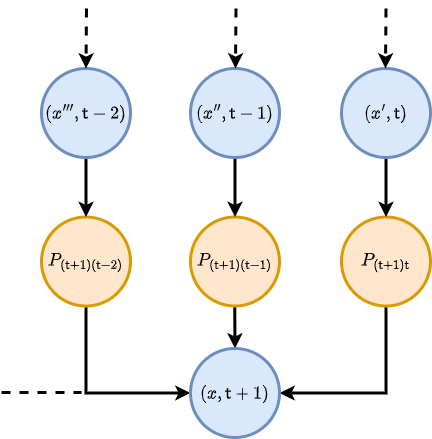
\includegraphics[width=8cm]{images/master-eq-graph.drawio.png}
\caption{Graph representation of Eq.~(\ref{eq:master-x-cont}).}
\label{fig:master-eqn}
\end{figure}

What if we wanted the joint distribution of both rows $P_{({\sf t}+1){\sf t}'}(x,x')$? One way to obtain this would be to extend Eq.~(\ref{eq:master-x-cont}) such that both matrix rows are marginalised over separately like so
%%
\begin{align}
&P_{({\sf t}+1){\sf t}'}(x,x') = \nonumber \\
&\qquad \frac{1}{({\sf t}'-1){\sf t}}\sum_{{\sf t}''=0}^{{\sf t}}\sum_{{\sf t}'''=0}^{{\sf t}'-1}\int_{\omega_{{\sf t}''}}{\rm d}x''\int_{\omega_{{\sf t}'''}}{\rm d}x''' P_{{\sf t}''{\sf t}'''}(x'', x''') P_{({\sf t}+1){\sf t}''}(x\vert x'')P_{{\sf t}'{\sf t}'''}(x'\vert x''') \label{eq:joint-master-x-cont} \,.
\end{align}
%%
Given Eqs.~(\ref{eq:master-x-cont}) and~(\ref{eq:joint-master-x-cont}) it's also possible to work out what the conditional probabilities would look like using the simple relation
%%
\begin{align}
P_{({\sf t}+1){\sf t}'}(x\vert x') &= \frac{P_{({\sf t}+1){\sf t}'}(x,x')}{P_{{\sf t}'}(x')} \label{eq:cond-master-x-cont} \,.
\end{align}
%%

The implicit notation in Eq.~(\ref{eq:master-x-cont}) can hide some staggering complexity. To analyse the system in more detail, we can also do a kind of Kramers-Moyal expansion~\cite{kramers1940brownian,moyal1949stochastic} for each point in time to approximate the overall equation like this
%%
\begin{align}
P_{{\sf t}+1}(x) &= \frac{1}{{\sf t}}\sum_{{\sf t}'=0}^{{\sf t}}P_{{\sf t}'}(x) - \frac{1}{{\sf t}}\sum_{{\sf t}'=0}^{{\sf t}}\sum_{i=1}^d\frac{\partial}{\partial x^i}\big[ \alpha^i_{({\sf t}+1){\sf t}'}(x)P_{{\sf t}'}(x)\big] \nonumber \\
& \qquad + \frac{1}{2{\sf t}}\sum_{{\sf t}'=0}^{{\sf t}}\sum_{i=1}^d\sum_{j=1}^d\frac{\partial}{\partial x^i}\frac{\partial}{\partial x^j}\big[ \beta^{ij}_{({\sf t}+1){\sf t}'}(x)P_{{\sf t}'}(x)\big] + \dots \label{eq:master-x-cont-kramers-moyal} \,,
\end{align}
%%
in which we have assumed that the state space is $d$-dimensional. In this expansion, we also needed to define these new integrals
%%
\begin{align}
\alpha^i_{({\sf t}+1){\sf t}'}(x) &=\int_{\omega_{{\sf t}'}} {\rm d}x'(x'-x)^iP_{({\sf t}+1){\sf t}'}(x'\vert x) \\
\beta^{ij}_{({\sf t}+1){\sf t}'}(x) &= \int_{\omega_{{\sf t}'}} {\rm d}x'(x'-x)^i(x'-x)^jP_{({\sf t}+1){\sf t}'}(x'\vert x) \,.
\end{align}
%%
So the matrix notation of Eq.~(\ref{eq:master-x-cont}) can indeed hide a very complicated calculation. Truncating the expansion at second-order, Eq.~(\ref{eq:master-x-cont-kramers-moyal}) tells us that there can be first and second derivatives contributing to the flow of probability to each element of the row $x=X_{{\sf t}+1}$ which depend on every element of the matrix $X'$. The probability does indeed \emph{flow}, in fact. We can define a quantity known as the `probability current' $J_{({\sf t}+1){\sf t}'}(x)$ from ${\sf t}'$ to $({\sf t}+1)$ which illustrates this through the following continuity relation
%%
\begin{align}
P_{{\sf t}+1}(x) - \frac{1}{{\sf t}}\sum_{{\sf t}'=0}^{{\sf t}}P_{{\sf t}'}(x) = \frac{1}{{\sf t}}\sum_{{\sf t}'=0}^{{\sf t}}\big[ P_{{\sf t}+1}(x) - P_{{\sf t}'}(x)\big] = - \frac{1}{{\sf t}}\sum_{{\sf t}'=0}^{{\sf t}}J_{({\sf t}+1){\sf t}'}(x) \,.
\end{align}
%%
By inspection of Eq.~(\ref{eq:master-x-cont-kramers-moyal}) we can therefore also deduce that
%%
\begin{align}
J^i_{({\sf t}+1){\sf t}'}(x) &= \alpha^i_{({\sf t}+1){\sf t}'}(x)P_{{\sf t}'}(x) - \frac{1}{2}\sum_{j=1}^d\frac{\partial}{\partial x^j}\big[ \beta^{ij}_{({\sf t}+1){\sf t}'}(x)P_{{\sf t}'}(x)\big] + \dots \,.
\end{align}
%%

What would happen if we assumed that $\alpha$ could be defined with just an arbitrary time-dependent function? In this instance, we mean
%%
\begin{align}
\alpha^i_{({\sf t}+1){\sf t}'}(x) &= f^i({\sf t}')-x^i \,,
\end{align}
%%
where $f({\sf t}')=f'$ is an arbitrary vector-valued function of the timestep. Using this function, we might then try to approximate $\beta^{ij}_{({\sf t}+1){\sf t}'}(x) \simeq \beta^{ij}_{({\sf t}+1){\sf t}'}(f') = 2K(\theta , {\sf t}' \vert f')$ with the matrix $K$, which depends on both the timestep and a set of hyperparameters $\theta$. If we now also assume stationarity of $P_{{\sf t}'}(x)=P_{{\sf t}''}(x)$ for any ${\sf t}'$ and ${\sf t}''$ such that
%%
\begin{align}
P_{{\sf t}+1}(x) = \frac{1}{{\sf t}}\sum_{{\sf t}'=0}^{{\sf t}} P_{{\sf t}'}(x) \,,
\end{align}
%%
we can solve Eq.~(\ref{eq:master-x-cont-kramers-moyal}) to obtain the following stationary solution
%%
\begin{align}
P_{{\sf t}'}(x) &= {\sf MultivariateNormalPDF}[x;f',K(\theta , {\sf t}' \vert f')]\label{eq:stat-sol-kramers-moyal}\,.
\end{align}
%%
Note in that last step the solution also required the identification that the flow of probability between timesteps vanishes uniquely for each and every ${\sf t}'$ such that $J_{({\sf t}+1){\sf t}'}(x)=0$. 

\begin{figure}[h]
\centering
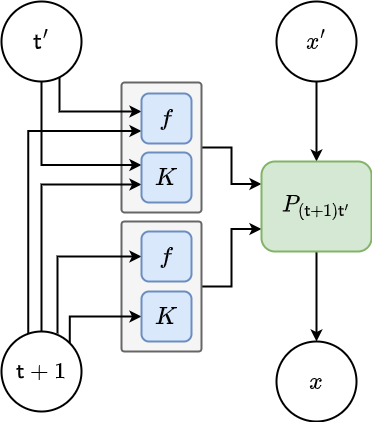
\includegraphics[width=8cm]{images/gp-like-diag.drawio.png}
\caption{Graph representation of the generative process implied by Eq.~(\ref{eq:stat-sol-kramers-moyal-cond}).}
\label{fig:stat-sol-kramers-moyal-cond}
\end{figure}

It's possible to take this derivation a bit further by expanding Eq.~(\ref{eq:joint-master-x-cont}) in a similar fashion, truncating it to second-order, assuming only time-dependent terms and then solving it in the stationary limit. By plugging this solution (and its corresponding marginal distribution equivalent) into Eq.~(\ref{eq:cond-master-x-cont}), you can get something that looks like this conditional distribution
%%
\begin{align}
P_{({\sf t}+1){\sf t}'}(x\vert x') &\propto {\rm exp}\bigg\{ -\frac{1}{2}\sum^d_{i=1}\sum^d_{j=1}(x-f)^i \big[K^{-1}(\theta , {\sf t}+1,{\sf t}+1\vert f,f)\big]^{ij}(x-f)^j \nonumber \\
& \qquad \qquad + \sum^d_{i=1}\sum^d_{j=1}(x-f)^i \big[ K^{-1}(\theta , {\sf t}+1,{\sf t}'\vert f,f')\big]^{ij}(x'-f')^j  \bigg\} \label{eq:stat-sol-kramers-moyal-cond}\,,
\end{align}
%%
where $f({\sf t}+1)=f$ and $K(\theta , {\sf t}+1,{\sf t}'\vert f,f')$ is some arbitrary covariance matrix that encodes how the correlation structure varies with the between compared states at two different timesteps and $K^{-1}$ denotes taking its inverse. Eq.~(\ref{eq:stat-sol-kramers-moyal-cond}) may look a bit familiar to some readers who like using Gaussian processes from the machine learning literature~\cite{murphy2012machine} --- this version implies a \emph{generative} model for a future $x$ value (which we've illustrated in Fig~\ref{fig:stat-sol-kramers-moyal-cond}), in contrast to the more standard equation used to \emph{infer} values of $f$. These are two sides of the same coin though. 

Written in Go, the conditional probability in Eq.~(\ref{eq:stat-sol-kramers-moyal-cond}) could be computed by performing the summations over each element of the state vectors. We've given a rough idea of what this code would look like below.

\begin{lstlisting}[language=Go]
import "math"

type KernelParams []float64

// returns the f function value for a given timestep
func F(timestepNumber int) []float64 {
    // return value
}

// returns the inverse-K matrix for the input timesteps and 
// params (theta in the text)
func inverseK(
    params KernelParams,
    timestepNumber int, 
    previousTimeStepNumber int,
) [][]float64 {
    // return value
}

// returns the conditional probability of the state vector at this timestep 
// given the value that the state vector had on a previous timestep
func StateVectorConditionalProbability(
    stateVector StateVector,
    timeStepNumber int,
    previousStateVector StateVector,
    previousTimeStepNumber int,
) float64 {
    // set the params from somewhere
    var kernelParams KernelParams
    
    // get the f-function values for both timesteps
    f := F(timeStepNumber)
    previousF := F(previousTimeStepNumber)
    
    // get the inverse-K matrices for the latest timestep
    // and also when both timesteps are input
    invK := inverseK(kernelParams, timeStepNumber, timeStepNumber)
    bothInvK := inverseK(
        kernelParams, 
        timeStepNumber, 
        previousTimeStepNumber,
    )

    // loop over terms to add to the log-probability
    logProbability := 0.0
    for i := range stateVector {
        for j := range stateVector {
            logProbability += -(stateVector[i] - f[i])*
                invK[i][j]*(stateVector[j] - f[j])/2.0
            logProbability += (stateVector[i] - f[i])*
                bothInvK[i][j]*(previousStateVector[j] - previousF[j])
        }
    }
    return math.Exp(logProbability)
}
\end{lstlisting}

By extending the procedure which obtains the joint distribution update in Eq.~(\ref{eq:joint-master-x-cont}) and uses Eq.~(\ref{eq:cond-master-x-cont}) to higher and higher orders of joint distribution $P_{({\sf t}+1){\sf t}'{\sf t}''}(x, x', x'')$, $P_{({\sf t}+1){\sf t}'{\sf t}''{\sf t}'''}(x, x', x'', x''')$, etc. you can derive equations for conditional distributions like $P_{({\sf t}+1){\sf t}'{\sf t}''}(x\vert x', x'')$ which are able to describe higher-order correlations between state vectors. Eq.~(\ref{eq:stat-sol-kramers-moyal-cond}) can hence be thought of as the second-order truncation of a more general expansion formula, similar to that of the Gram-Charlier A series, Edgeworth series~\cite{kolassa2006series}. The problem you have to look out for when using the higher-order terms in these series is that it's quite possible to define a probability distribution with them that does not converge to a finite normalisation when integrating over its entire domain. To avoid this issue, the kind of expansion that we shall perform instead leverages a derivative approximation of $K$ and is known as the DALI method~\cite{sellentin2014breaking, dali}. In our case, this derivative approximation manifests as an expansion of $K$ to include higher-order dependencies on $x''$ and $x'''$ like so\footnote{Another way of thinking about this approximation is that it is a `mean-field' expansion of the covariance matrix to include higher-order terms.}
%%
\begin{align}
& K(\theta , {\sf t}+1, {\sf t}', {\sf t}'', {\sf t}'''\vert f,f',x'',x''') \simeq \nonumber \\
& K + \sum_{i=1}^d(x''-f'')^i\frac{\partial K}{(\partial x'')^i} + \sum_{i=1}^d(x'''-f''')^i\frac{\partial K}{(\partial x''')^i} + \frac{1}{2}\sum_{i=1}^d\sum_{j=1}^d (x''-f'')^i\frac{\partial^2 K}{(\partial x'')^i(\partial x'')^j}(x''-f'')^j \nonumber \\
&+ \frac{1}{2}\sum_{i=1}^d\sum_{j=1}^d (x'''-f''')^i\frac{\partial^2 K}{(\partial x''')^i(\partial x''')^j}(x'''-f''')^j + \sum_{i=1}^d\sum_{j=1}^d (x''-f'')^i\frac{\partial^2 K}{(\partial x'')^i(\partial x''')^j}(x'''-f''')^j \,,
\end{align}
%%
where all of the references to `$K$' above are evaluated using $x=f$, $x'=f'$, $x''=f''$ and $x'''=f'''$ after any derivatives of the variable have been taken.

Note that that the version of the DALI method that we have described here is in a different context to where it has been employed in the literature. In our case, the probability distribution that we are trying to approximate contains out-of-time-order correlations in a similar fashion to those studied in quantum mechanics~\cite{hashimoto2017out,García-Mata:2023} (though we are obviously only talking about a classical statistical analogue in this case). 

Hence, if $K(\theta, {\sf t}+1, {\sf t}')$ is a matrix which encodes second-order (pairwise) out-of-time order correlations, we shall denote the higher-rank\footnote{By `higher-rank' here we specifically mean objects which have more indices than just a matrix $M^{ij}\rightarrow M^{ijk\dots}$.} objects which encode higher-order correlations between state vectors at different time points as
%%
\begin{align}
\ K(\theta , {\sf t}+1, {\sf t}', {\sf t}'') \quad &\text{with elements} \quad K^{ijk}(\theta , {\sf t}+1, {\sf t}', {\sf t}'') \label{eq:third-prob-kernel} \\
\ K(\theta , {\sf t}+1, {\sf t}', {\sf t}'', {\sf t}'''') \quad &\text{with elements} \quad K^{ijk\ell}(\theta , {\sf t}+1, {\sf t}', {\sf t}'', {\sf t}''') \label{eq:fourth-prob-kernel} \,,
\end{align}
%%
and so on until the desired order of truncation is reached.

Despite these expressions appearing as more complex than the second-order version, the methology for using them in a generative model like Eq.~(\ref{eq:stat-sol-kramers-moyal-cond}), or for levering them to infer the $f({\sf t})$ function (as is done in Gaussian process inference) is much the same. 

What other processes can be described by Eq.~(\ref{eq:master-x-cont})? For Markovian phenomena, the equation no longer depends on timesteps older than the immediately previous one, hence the expression reduces to just
%%
\begin{align}
P_{{\sf t}+1}(x) &= \int_{\omega_{\sf t}}{\rm d}x' P_{\sf t}(x') P_{({\sf t}+1){\sf t}}(x\vert x') \label{eq:master-x-cont-markov} \,.
\end{align}
%%
It's also easy to show that Eq.~(\ref{eq:master-x-cont-kramers-moyal}) naturally simplifies into the more usually applied Kramers-Moyal expansion when considering a Markovian process --- you just remove the sum over ${\sf t}'$ and the $1/{\sf t}$ normalisation factor. 

Note that an analog of Eq.~(\ref{eq:master-x-cont}) exists for discrete state spaces as well. We just need to replace the integral with a sum and the schematic would look something like this
%%
\begin{align}
P_{{\sf t}+1}(x) &= \frac{1}{{\sf t}}\sum_{{\sf t}'=0}^{\sf t}\sum_{\omega_{{\sf t}'}} P_{{\sf t}'}(x') P_{({\sf t}+1){\sf t}'}(x \vert x') \label{eq:master-x-disc} \,,
\end{align}
%%
where we note that the $P$'s in the expression above all now refer to \emph{probability mass functions}. Because the state space is now discrete, we cannot immediately intuit an approximative expansion from this expression. 

As a brief mathematical aside; if you're really determined to use a similar approach to the one we derived above, you can rewrite it in terms of continuous-valued characteristic functions like this
%%
\begin{align}
\varphi_{{\sf t}+1}(s) &= \frac{1}{{\sf t}}\sum_{{\sf t}'=0}^{\sf t}\int_{\ell_{{\sf t}'}}{\rm d}s' {\cal C}(s') \varphi_{{\sf t}'}(s') \varphi_{({\sf t}+1){\sf t}'}(s \vert s') \label{eq:master-x-disc-char} \\
{\cal C}(s') &= \frac{1}{(2\pi )^d}\sum_{\omega_{{\sf t}'}}e^{-i(s'\cdot x')} \,,
\end{align}
%%
where $\ell_{{\sf t}'}$ defines all the continuous values that the vector $s'$ can possibly have at time ${\sf t}'$. In the expression above, ${\cal C}(s')$ acts like is a kind of comb\footnote{This is very similar to how a `Dirac comb' works in signal processing~\cite{brandwood2012fourier}.} to map the continuous frequency domain of $s'$ onto the discrete state space of $x'$. Note also that ${\cal C}(s')$ uses the imaginary number $i$ and, to be visually tidier, the dot product notation $a\cdot b$ just means the sum of vector elements: $a\cdot b = \sum_{\forall k}a^kb^k$. In principle, one can perform an approximative expansion on Eq.~(\ref{eq:master-x-disc-char}) like we did for continuous state spaces. This isn't always the most practical way of analysing the system though. 

We have one more important example to discuss and then we can cap off this more mathematical section. In the even-simpler case where $x$ is just a vector of binary `on' or `off' states, Eq.~(\ref{eq:master-x-disc}) reduces to
%%
\begin{align}
P^i_{{\sf t}+1} &= \frac{1}{{\sf t}}\sum_{{\sf t}'=0}^{\sf t} \sum_{j=1}^d P^j_{{\sf t}'} P^{ij}_{({\sf t}+1){\sf t}'} = \frac{1}{{\sf t}}\sum_{{\sf t}'=0}^{\sf t} \sum_{j=1}^d \big[ P^j_{{\sf t}'} A^{ij}_{({\sf t}+1){\sf t}'} + (1-P^j_{{\sf t}'}) B^{ij}_{({\sf t}+1){\sf t}'} \big] \label{eq:master-x-disc-binary}\,,
\end{align}
%% 
where $P^i_{{\sf t}'}$ now represents the probability that element $x^i=1$ (is `on') at time ${\sf t}'$. The matrices $A$ and $B$ are defined as conditional probabilities where the previous state in time $P^j_{{\sf t}'}$ was either `on' or `off', respectively.

In this section, we looked into how the mathematical formalism used in the stochadex could be extended with probability theory. Now that we have more of a sense of how this formalism works, we are ready to move on to designing the algorithms for our emulator. So let's go!

\section{\sffamily Emulator algorithms}

Plan of action for this section.
\begin{itemize}
\item{Introduce the concept of retrieving state data through measurements $Y^i_{{\sf t}+1} = M^i_{{\sf t}+1}(X_{{\sf t}+1},z,{\sf t})$.}
\item{Parametric algorithm will be available up to 4th order expansion. This should just be a straightforward optimisation.}
\item{Non-parametric algorithm concept will be just for Gaussian processes and will use a secondary kernel applied to the non-parametric kernel shape + EM algorithm.}
\end{itemize}

The parametric algorithm simply needs the $K$-functions to be specified and then an optimiser can run over the data values to simultaneously attempt to obtain $\theta$ and $f$ values.

For the full non-parametric algorithm, the best idea here is probably to write a kind of Expectation-Maximisation (EM) algorithm. This would be...

Estimating what $K(\theta , {\sf t}, {\sf t}')$, $K(\theta , {\sf t}, {\sf t}', {\sf t}'')$ and $K(\theta , {\sf t}, {\sf t}', {\sf t}'', {\sf t}''')$ should all look like based on a history of data values $y,y',\dots$ measured at times $t,t',\dots$ and a proposed set of $f,f'.\dots$ function values where we are using, e.g., $t'=t({\sf t}')$ and $f'=f({\sf t}')$ as a shorthand for convenience. We can do this using estimates for the 2, 3 and 4-point temporal correlation coefficients, which are
%%
\begin{align}
{\rm Corr}(y,t;y',t') &= \frac{{\rm E}[(y-f)(y'-f')]}{[{\rm Var}(y){\rm Var}(y')]^{1/2}} \\
{\rm Corr}(y,t;y',t';y'',t'') &= \frac{{\rm E}[(y-f)(y'-f')(y''-f'')]}{[{\rm Var}(y){\rm Var}(y'){\rm Var}(y'')]^{1/3}} \\
{\rm Corr}(y,t;y',t';y'',t'';y''',t''') &= \frac{{\rm E}[(y-f)(y'-f')(y''-f'')(y'''-f''')]}{{[{\rm Var}(y){\rm Var}(y'){\rm Var}(y''){\rm Var}(y''')]^{1/4}}} \,.
\end{align}
%%
And then using these correlation coefficients as weightings to non-parametrically construct a set of $K$-functions. Hyperparameters to help with learning on this step include the order $K$-function to go up to (maximum of 4th order) and also maybe a minimum value for the correlation coefficient in order for it to be included? This concludes the `Expectation' step.

Once the $K$-functions have been estimated for this step, an optimiser algorithm can be run using them and the formula for the log-likelihood to find out what the optimal $f$ value is as a function of $t({\sf t})$. This is the `Maximisation' step.

The steps above are then run in an alternating fashion until convergence. 

Helpful to write the basic structure out in Go.

\section{\sffamily Software design}

